\chapter{Einige wichtige Hinweise zum Arbeiten mit \LaTeX\ }
\label{sec:latexumg}

Nachfolgend wird die Codierung einiger oft verwendeten Elemente
kurz beschrieben. Das Einbinden von Bildern ist in \LaTeX\ nicht
ganz unproblematisch und hängt auch stark vom verwendeten Compiler
ab. Typisches Format für Bilder in \LaTeX\ ist
EPS\footnote{Encapsulated Postscript} oder PDF\footnote{Portable Document Format}.

\section{Basics}
\label{sec:basics}
Text kann durch die Befehle \texttt{\textbackslash textit} (\textit{italic}), \texttt{\textbackslash texttt}  (\texttt{typewriter}) und \texttt{\textbackslash textbf} (\textbf{bold}) formatiert werden. Zeilenumbrüche im Text werden auch im PDF übernommen. Um eine leere Zeile einzufügen muss ein Zeilenumbruch (\textbackslash \textbackslash) hinzugefügt werden.\\

Um Position weiter zu beeinflussen können die Befehle für \texttt{\textbackslash vspace[Distanz]} und \texttt{\textbackslash hspace[Distanz]} benutzt werden.
Es können auch Kommentare im Code eingefügt werden mit \texttt{\%}.

\section{Gliederungen}
\label{sec:gliederung}

Ein Text kann mit den Befehlen \texttt{\textbackslash
chapter\{.\}}, \texttt{\textbackslash section\{.\}},
\texttt{\textbackslash subsection\{.\}} und \texttt{\textbackslash
subsubsection\{.\}} gegliedert werden. Weiterhin kann das ganze Dokument in verschiedene Dateien gegliedert werden, welche durch den Befehl \texttt{\textbackslash input\{.\}} eingefügt werden können.


\section{Referenzen und Verweise}
\label{sec:refverw}

Literaturreferenzen werden mit dem Befehl \texttt{\textbackslash
citep\{.\}} und \texttt{\textbackslash
citet\{.\}} erzeugt. Beispiele: ein Buch \citep{Raibert1986LeggedRobotsThatBalance}, ein Buch und ein Journal Paper \citep{Raibert1986LeggedRobotsThatBalance,Vukobratovic2004ZeroMomentPoint}, ein Konferenz Paper mit Erwähnung des Autors: \citet{Pratt1995SEA}.

Zur Erzeugung von Fussnoten wird der Befehl \texttt{\textbackslash
footnote\{.\}} verwendet. Auch hier ein Beispiel\footnote{Bla
bla.}.

Bibliografieeinträge können einfach falls vorhanden von den jeweiligen Seiten eingefügt werden, mit dem Program Jabref\footnote{https://www.jabref.org}, welches auch eine Suchmaschine beiinhaltet, generiert werden oder von Hand selber hinzugefügt werden. Dabei ist auf die Aufzählung der Autoren zu achten, welche immer mit einem trennenden \texttt{and} hinzugefügt werden müssen. 

Querverweise im Text werden mit \texttt{\textbackslash label\{.\}}
verankert und mit \texttt{\textbackslash cref\{.\}} erzeugt.
Beispiel einer Referenz auf das zweite Kapitel:
\cref{sec:latexumg}.


\section{Aufzählungen}\label{sec:aufz}

Folgendes Beispiel einer Aufzählung ohne Numerierung,
\begin{itemize}
  \item Punkt 1
  \item Punkt 2
\end{itemize}
wurde erzeugt mit:
\begin{verbatim}
\begin{itemize}
  \item Punkt 1
  \item Punkt 2
\end{itemize}
\end{verbatim}

Folgendes Beispiel einer Aufzählung mit Numerierung,
\begin{enumerate}
  \item Punkt 1
  \item Punkt 2
\end{enumerate}
wurde erzeugt mit:
\begin{verbatim}
\begin{enumerate}
  \item Punkt 1
  \item Punkt 2
\end{enumerate}
\end{verbatim}

Folgendes Beispiel einer Auflistung,
\begin{description}
  \item[P1] Punkt 1
  \item[P2] Punkt 2
\end{description}
wurde erzeugt mit:
\begin{verbatim}
\begin{description}
  \item[P1] Punkt 1
  \item[P2] Punkt 2
\end{description}
\end{verbatim}


\section{Erstellen einer Tabelle}\label{sec:tabellen}

Ein Beispiel einer Tabelle (siehe \Cref{tab:tabnefz}).
\begin{table}[ht]
\begin{center}
 \caption{Daten der Fahrzyklen ECE, EUDC, NEFZ.}\vspace{1ex}
 \label{tab:tabnefz}
 \begin{tabular}{ll|ccc}
 \hline
 Kennzahl & Einheit & ECE & EUDC & NEFZ \\ \hline \hline
 Dauer & s & 780 & 400 & 1180 \\
 Distanz & km & 4.052 & 6.955 & 11.007 \\
 Durchschnittsgeschwindigkeit & km/h & 18.7 &  62.6 & 33.6 \\
 Leerlaufanteil & \% & 36 & 10 & 27 \\
 \hline
 \end{tabular}
\end{center}
\end{table}

Die Tabelle wurde erzeugt mit:
\begin{verbatim}
\begin{table}[ht]
\begin{center}
 \caption{Daten der Fahrzyklen ECE, EUDC, NEFZ.}\vspace{1ex}
 \label{tab:tabnefz}
 \begin{tabular}{ll|ccc}
 \hline
 Kennzahl & Einheit & ECE & EUDC & NEFZ \\ \hline \hline
 Dauer & s & 780 & 400 & 1180 \\
 Distanz & km & 4.052 & 6.955 & 11.007 \\
 Durchschnittsgeschwindigkeit & km/h & 18.7 &  62.6 & 33.6 \\
 Leerlaufanteil & \% & 36 & 10 & 27 \\
 \hline
 \end{tabular}
\end{center}
\end{table}
\end{verbatim}


\section{Einbinden einer Grafik}\label{sec:epsgraph}

Das Einbinden von Graphiken kann wie folgt bewerkstelligt werden:
\begin{verbatim}
\begin{figure}[hbp]
   \centering
   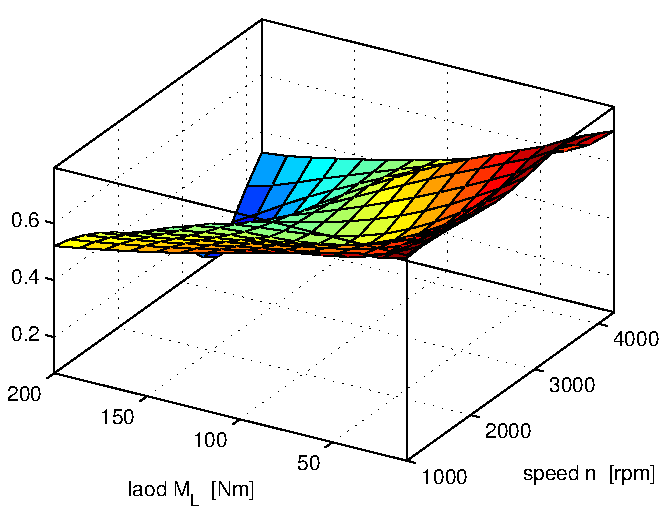
\includegraphics[width=0.75\textwidth]{images/k_surf.pdf}
   \caption{Ein Bild.}
   \label{fig:k_surf}
\end{figure}
\end{verbatim}

\begin{figure}[hbp]
   \centering
   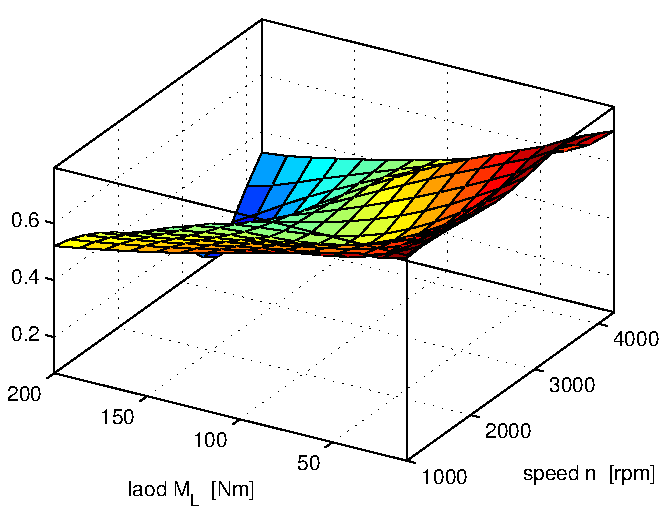
\includegraphics[width=0.75\textwidth]{images/k_surf.pdf}
   \caption{Ein Bild}
   \label{pics:k_surf}
\end{figure}

Das $\lbrack hbp \rbrack$ macht, dass das Bild entweder an dieser Stelle im Layout eingebettet wird, wenn das nicht geht am Ende der Seite und wenn dies auch nicht geht, am Ende der nächsten Seite. Referenzieren der Bilder geht am besten mit \texttt{\textbackslash Cref\{.\}} (\Cref{pics:cycle:1}) oder \texttt{\textbackslash cref\{.\}} (\cref{pics:cycle:1}).\\

Zwei Bilder nebeneinander einfügen mit:

\begin{verbatim}
\begin{figure}[hbp]
  \begin{subfigure}[t]{0.48\textwidth}
    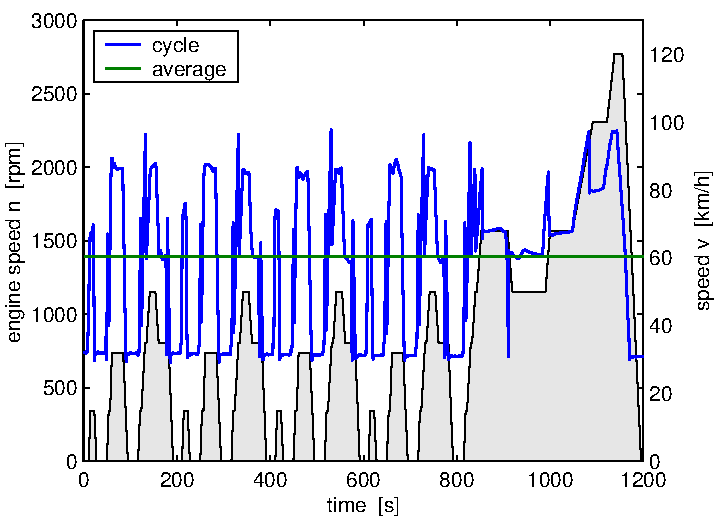
\includegraphics[width = \textwidth]{images/cycle_we.pdf}
    \caption{Bild 1}
    \label{pics:cycle:1}
  \end{subfigure}
  \hfill
  \begin{subfigure}[t]{0.48\textwidth}
    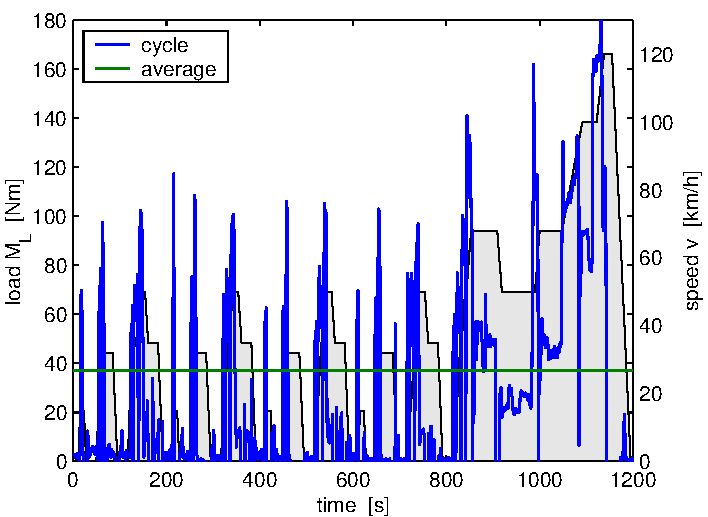
\includegraphics[width = \textwidth]{images/cycle_ml.pdf}
    \caption{Bild 2}
    \label{pics:cycle:2}
  \end{subfigure}
  \caption{Zwei Bilder nebeneinander}
  \label{pics:cycle}
\end{figure}
\end{verbatim}

\begin{figure}[hbp]
  \begin{subfigure}[t]{0.48\textwidth}
    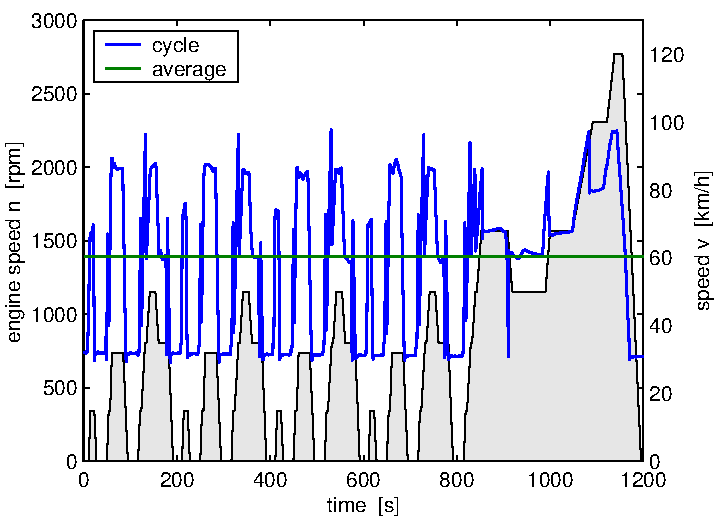
\includegraphics[width = \textwidth]{images/cycle_we.pdf}
    \caption{Bild 1}
    \label{pics:cycle:1}
  \end{subfigure}
  \hfill
  \begin{subfigure}[t]{0.48\textwidth}
    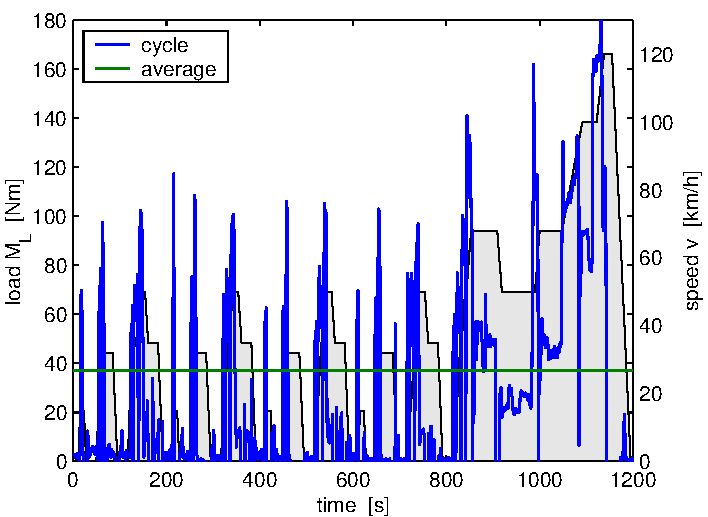
\includegraphics[width = \textwidth]{images/cycle_ml.pdf}
    \caption{Bild 2}
    \label{pics:cycle:2}
  \end{subfigure}
  \caption{Zwei Bilder nebeneinander}
  \label{pics:cycle}
\end{figure}

Tikz ist kein Zeichnungsprogramm, aber ein praktisches Tool um inline in Latex Dokumenten Vektorgrafiken zu erstellen (see \Cref{fig:loop}). Viele weitere Möglichkeiten findest du in der Dokumentation\footnote{https://mirror.kumi.systems/ctan/graphics/pgf/base/doc/pgfmanual.pdf}.

\begin{figure}[hbp]
\begin{center}
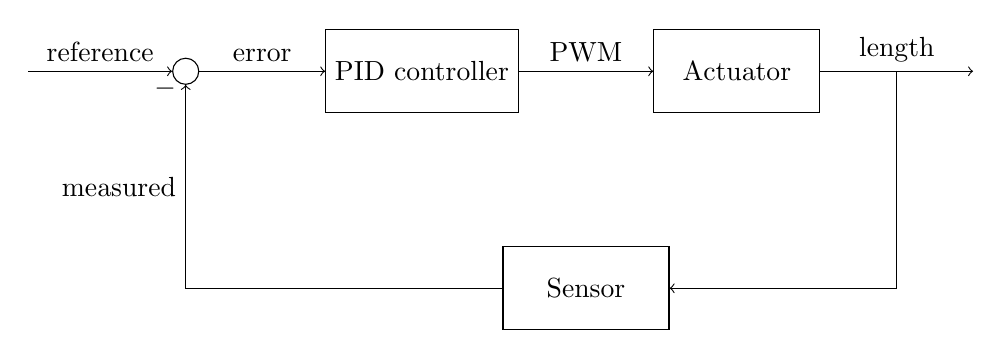
\begin{tikzpicture}[auto, node distance=3cm]
    \tikzstyle{block} = [draw, fill=white, rectangle, 
    minimum height=3em, minimum width=6em]
    \tikzstyle{sum} = [draw, fill=white, circle, node distance=1cm]
    \tikzstyle{input} = [coordinate]
    \tikzstyle{output} = [coordinate]
    \tikzstyle{pinstyle} = [pin edge={to-,thin,black}]
    \node [input, name=input]{};
    \node[sum, right of=input, node distance=2cm](sum){};
    \node [block, right of=sum](controller){PID controller};
    \node [block, right of=controller, node distance=4cm](system){Actuator};
    \draw [->] (controller) -- node[name=u]{PWM}(system);
    \node [output, right of=system, node distance=3cm](output) {};
    \node [block, below of=u](measurements){Sensor};
    \draw [draw,->] (input) -- node [align=center]{reference}(sum);
    \draw [->] (sum) -- node {error}(controller);
    \draw [->] (system) -- node [name=y]{length}(output);
    \draw [->] (y) |- (measurements);
    \draw [->] (measurements) -| node[pos=0.99] {$-$} 
        node [near end, align=center]{measured}(sum);
\end{tikzpicture}
\caption{Ein Beispiel von Tikz} \label{fig:loop}

\end{center}
\end{figure}






\section{Mathematische Formeln}\label{sec:math}

Einfache mathematische Formeln werden mit der equation-Umgebung
erzeugt:
\begin{equation}
 p_{me0f}(T_e,\omega_e) \ = \ k_1(T_e) \cdot (k_2+k_3 S^2
 \omega_e^2) \cdot \Pi_{\mathrm{max}} \cdot \sqrt{\frac{k_4}{B}} \quad [\text{bar}] .
 	\label{eq:my_equation}
\end{equation}

Der Code dazu lautet:
\begin{verbatim}
\begin{equation}
 p_{me0f}(T_e,\omega_e) \ = \ k_1(T_e) \cdot (k_2+k_3 S^2
 \omega_e^2) \cdot \Pi_{max} \cdot \sqrt{\frac{k_4}{B}} \quad [\text{bar}] .
\end{equation}
\end{verbatim}

Mathematische Ausdrücke im Text werden mit \$formel\$ erzeugt (z.B.:
$a^2+b^2=c^2$).

Vektoren und Matrizen werden mit den Befehlen \texttt{\textbackslash vec\{.\}} und \texttt{\textbackslash mat\{.\}} erzeugt (z.B. $\vec{v}$, $\mat{M}$). Matrizen kann man aber auch explizit in Formeln verwenden. Bsp:

\begin{equation}
    \begin{bmatrix}
    1 & 2 \\
    3 & 4 
    \end{bmatrix}
    \begin{bmatrix}
    1 \\
    1
    \end{bmatrix}
    = 
    \begin{bmatrix}
    3 \\
    7
    \end{bmatrix}
    \vspace{0.5cm}
\end{equation}

Um Text, oder unformatierte Zeichen in Gleichungen eizufügen braucht man eine Textumgebung \texttt{\textbackslash text\{.\}}.

Leerzeichen in Gleichungen erhält man durch \texttt{\textbackslash,} und grössere mit
\texttt{\textbackslash quad} oder \texttt{\textbackslash qquad}.


\section{Weitere nützliche Befehle}\label{sec:div}

Hervorhebungen im Text sehen so aus: \emph{hervorgehoben}. Erzeugt
werden sie mit dem \texttt{\textbackslash epmh\{.\}} Befehl.

Einheiten werden mit den Befehlen \texttt{\textbackslash unit[1]\{m\}} (z.B.~\unit[1]{m}) und \texttt{\textbackslash unitfrac[1]\{m\}\{s\}} (z.B.~\unitfrac[1]{m}{s}) gesetzt. Alternativ kann auch bei einfachen Einheiten ein Umbruchgeschütztes Leerzeichen verwendet werden: \texttt{1 \textbackslash , m} (1\,m).

\subsection{Tiefe der Gliederung}
Dies ist ein Abschnitt auf der dritten Hierarchistufe.

\subsubsection{Zwischentitel}
Dies ist ein Abschnitt auf der vierten Hierarchistufe. Diese ist unnummeriert und geht nicht ins Inhaltsverzeichnis ein.